% !TEX program = pdflatex
\documentclass[sigconf,anonymous,review,balance=false]{acmart}

\usepackage{graphicx}
\usepackage{booktabs}
\usepackage{microtype}
\usepackage{multirow}
\usepackage{enumitem}
\usepackage{array}
\usepackage{subcaption}
\usepackage{tabularx}
\usepackage{float}
\usepackage{placeins}
\usepackage{amsmath}
\let\Bbbk\relax
\usepackage{amssymb}
\usepackage{listings}
\usepackage{xcolor}

\settopmatter{printacmref=false,printccs=false}
\setcopyright{none}
\renewcommand\footnotetextcopyrightpermission[1]{}

\acmConference[KDD '27]{The 33rd ACM SIGKDD Conference on Knowledge Discovery and Data Mining}{August 1--5, 2027}{San Jose, CA, USA}
\acmISBN{}
\acmDOI{}
\acmYear{2027}
\copyrightyear{2027}

\newcommand{\clip}{\operatorname{clip}}
\newcommand{\sigmoid}{\operatorname{sigmoid}}
\newcommand{\ind}{\mathbf{1}}

\AtBeginDocument{%
  \providecommand\BibTeX{{Bib\TeX}}}

\newcommand{\tr}[2]{#2}
\emergencystretch=1em
\begin{document}

\title[Civitas Economica: Multi-Scale Market Simulation]{Civitas Economica: An Interdisciplinary LLM Agent-Based Market Simulation Architecture for Multi-Scale Socio-Economic Dynamics}

\begin{abstract}
Civitas Economica is an agent-based market simulator that supports large language model (LLM) agents. It models how economic relations evolve between investors, between an investor and a group, and between the group and market institutions. Social psychology motivates attention, panic contagion, and confidence-dependent herding. Behavioral finance connects portfolios and multiple price references to valuation. Game theory motivates the interdependence arising from shared information, prices, and trading constraints. A discrete causal clock and a continuous double auction couple these mechanisms to integer settlement. Numerical rules, persona heuristics, LLM agents, and a dual-speed scheduler share the same order contract. In branches from one parent world, suppressing secondary contagion lowers peak infection from 45\% to 5\% and maximum drawdown from 0.4754\% to 0.1453\%. Removing herding changes turnover, and the contagion--herding interaction on drawdown is zero in this world. A halt shows why price paths must be read alongside access to matching. Intraday trajectories and fixed-observation LLM requests exercise the market and decision interfaces. The simulator makes it possible to follow changes in an investor's state through group dynamics and market institutions back to subsequent decisions.
\end{abstract}

\keywords{Agent-Based Social Simulation, Behavioral Finance, Social Contagion, LLM Agents, Strategic Interdependence, Market Microstructure}

\maketitle

\section{Introduction}
\label{sec:introduction}

A last-trade price records the most recent match. Between matches, investors can receive new information, revise their trading intentions, and change how much weight they give to peers. Explaining a price response to a shock therefore requires knowing when the market could trade, how investors responded to one another, and which information reached their decisions. Agent-based models link interactions of this kind to emergent market statistics~\cite{cont2001empirical,lebaron2006agent,farmer2009economy,lux1999scaling}. Our question is how to make the economic relations between investors, groups, and the market explicit enough to study them in a single simulation.

\textbf{Civitas Economica} organizes those relations at three scales (Figure~\ref{fig:overview}).
\begin{itemize}[leftmargin=*,itemsep=2pt]
 \item \textbf{Person to person.} An investor's portfolio links financial risk to social contact. On a fixed network, investors with similar risk exposure receive stronger relative ties. Limited attention determines which messages reach each investor.
 \item \textbf{Person to group.} Exposure to peers can propagate panic. The prevalence of pessimism and an investor's own confidence govern reliance on the group. Investor archetypes provide heterogeneous mandates and decision parameters, and the group state evolves through network interaction.
 \item \textbf{Group to society.} Orders from the population meet in a continuous double auction. Trading rules determine which orders can execute, and settled trades produce prices, holdings, and liquidity that feed into the next step. This scale represents the collective outcomes of the modeled market.
\end{itemize}

The design draws on social psychology to model attention, emotional contagion, and conformity~\cite{deutsch1955study,hatfield1993emotional,tajfel1979integrative}, and on behavioral finance to connect holdings and price references to valuation~\cite{kahneman1979prospect,tversky1992advances}. Game theory motivates the focus on strategic interdependence because one investor's actions can change the information, prices, and constraints faced by others~\cite{cooper1988coordinating,keynes1936general,morris2002social}. The simulator expresses these channels as behavioral updates and exchange rules. It uses a common observation and order contract to accommodate numerical rules, persona heuristics, full LLM agents, and a dual-speed policy in this loop.

\subsection{Research Questions}
\label{sec:rq}

\begin{itemize}[leftmargin=*,itemsep=3pt]
 \item \textbf{Market activity (RQ1).} How do behavioral rules affect trading activity and quote availability under the same exchange rules and sparse activation?
 \item \textbf{Feedback across scales (RQ2).} From a common market state, how do panic propagation, confidence-dependent herding, valuation, and regulatory rules change social states, prices, and trading opportunities?
 \item \textbf{Decision interfaces and scheduling (RQ3).} How do the supported decision backends respond to changes in price, locked inventory, and cash in fixed observations? How does a periodic LLM schedule trade off request opportunities and access to an event message?
\end{itemize}

\subsection{Main Contributions}
\label{sec:contributions}

\begin{itemize}[leftmargin=*,itemsep=2pt]
 \item \textbf{An explicit model of economic relations across three scales.} Portfolio exposure shapes social ties, group states affect valuation and order intent, and market clearing changes the prices and portfolios that agents carry forward.
 \item \textbf{A common execution environment for heterogeneous agents.} A causal clock defines when information becomes visible. The integer ledger tracks reservations and transfers under the same market rules for each decision backend. The dual-speed policy caches a direction and a resource fraction so the next order can use current prices and balances.
 \item \textbf{Observable comparisons of the three scales.} Shared checkpoints let us change an interaction or market rule and trace the responses from social states to trades. The diagnostics combine those paths with intraday liquidity records, persona-level action contrasts, and measured runtime.
\end{itemize}

\section{Related Work}
\label{sec:related}

\subsection{Behavioral Finance and Social Relations}

Prospect theory describes reference dependence, loss aversion, and diminishing sensitivity~\cite{kahneman1979prospect,tversky1992advances}. Mental accounting and endogenous references explain how one price can be assessed against different benchmarks~\cite{thaler1985mental,koszegi2006model}. The disposition effect motivates tracking acquisition costs separately from current prices~\cite{shefrin1985disposition,odean1998reluctant}. Civitas connects these financial states to person-to-person relations through portfolio-exposure similarity. Acquisition cost, recent highs, peer consensus, and policy signals enter reference-dependent valuation.

Social psychology studies group affiliation, emotional contagion, and informational and normative influence~\cite{tajfel1979integrative,hatfield1993emotional,deutsch1955study}. Small-world connectivity and selective exposure motivate the contact network and access to information~\cite{watts1998collective,sunstein2001republic}. At the person-to-group scale, Civitas uses attention-bounded message selection and synchronous panic transitions to update local social states. Confidence controls the weight placed on peers. Investor archetypes specify heterogeneous roles independently of network position. The modeled group feedback arises through neighborhood interaction.

\subsection{Coordination and Market Institutions}

Strategic complementarities, expectations about others' valuations, and public-information games describe incentives to coordinate~\cite{cooper1988coordinating,keynes1936general,morris2002social}. Information-cascade models explain how earlier actions influence later decisions~\cite{bikhchandani1992theory,banerjee1992simple}. Noise-trader risk and limits to arbitrage explain why price deviations can persist~\cite{delong1990noise,shleifer1997limits}. These theories motivate peer-dependent updates in Civitas, which evolves its specified behavioral rules forward in time. Its group-to-society scale is the modeled market institution, where collective orders produce prices and trading opportunities that feed back into individual decisions.

Exchange design governs this aggregation. Zero-intelligence experiments isolate the contribution of budget constraints and double-auction rules~\cite{gode1993allocative}. Interacting chartist and fundamentalist models generate heavy tails and volatility clustering~\cite{lux1999scaling,lux2000volatility,raberto2001agent}. Microstructure theory links price formation to information asymmetry~\cite{kyle1985continuous,glosten1985bid}. ABIDES provides a discrete-event limit order book with configurable communication delays and programmable agents~\cite{abides2020}. Civitas uses discrete decision barriers followed by sequential order arrivals at a continuous double auction, with a common information boundary before matching.

\subsection{Language Models in Market Simulations}

Generative agents interpret observations and enact roles through language~\cite{park2023generative}. Financial applications include layered memory in FinMem, multimodal signals and tools in FinAgent, and role-based trading in StockAgent and TradingAgents~\cite{yu2023finmem,zhang2024finagent,li2024stockagent,xiao2024tradingagents}. EconAgent models household labor and consumption~\cite{li2024econagent}. TwinMarket couples belief--desire--intention investors and social information to a call auction~\cite{yang2025twinmarket}. MarketSim separates strategic LLM decisions from high-frequency execution in a continuous double auction~\cite{marketsim2026}. StockSim provides order-level LLM evaluation with two execution settings, latency, and slippage~\cite{papadakis2025stocksim}.

Table~\ref{tab:related_comparison} separates exchange design, social and behavioral mechanisms, decision organization, and evaluation focus. Civitas combines independently adjustable social and valuation rules with integer accounting and branches from a shared state. The comparison follows changes from interpersonal exposure and group feedback to order intent and execution under a common decision contract.

\begin{table*}[t]
  \centering\small
  \setlength{\tabcolsep}{4pt}
  \caption{\tr{金融市场仿真平台的设计与评估重点。各项概括所引文献报告的功能与研究重点。}{Design and evaluation focus of financial market simulators. Entries summarize features and study emphases reported in the cited work.}}
  \label{tab:related_comparison}
  \begin{tabularx}{\textwidth}{@{}>{\raggedright\arraybackslash}p{1.95cm} >{\raggedright\arraybackslash}p{2.65cm} >{\raggedright\arraybackslash}p{3.5cm} >{\raggedright\arraybackslash}p{3.3cm} >{\raggedright\arraybackslash}X@{}}
    \toprule
    \tr{平台}{Platform} & \tr{交易机制}{Exchange} & \tr{社会与行为机制}{Social / behavioral layer} & \tr{决策组织}{Decision organization} & \tr{评估与审计重点}{Evaluation and audit focus} \\
    \midrule
    \textbf{ABIDES}\newline\cite{abides2020} & \tr{离散事件限价订单簿；通信延迟}{Discrete-event limit order book; communication latency} & \tr{背景交易者与策略交易者}{Background and strategic traders} & \tr{可编程主体策略}{Programmable agent policies} & \tr{订单与消息记录；交易实验}{Order and message traces; trading experiments} \\
    \addlinespace
    \textbf{TwinMarket}\newline\cite{yang2025twinmarket} & \tr{日级集合竞价}{Daily call auction} & \tr{交易相似度社会信息流；谣言传播}{Trading-similarity social feed; rumor diffusion} & \tr{基于信念--愿望--意图的 LLM 投资者}{Belief--desire--intention LLM investors} & \tr{风格化事实与社会响应场景}{Stylized facts and social-response scenarios} \\
    \addlinespace
    \textbf{MarketSim}\newline\cite{marketsim2026} & \tr{纳秒精度连续双向拍卖}{Nanosecond-resolution continuous double auction} & \tr{异质投资者；新闻与政策信息}{Heterogeneous investors; news and policy information} & \tr{战略层 LLM 决策与快速执行层}{Strategic LLM decisions with a faster execution layer} & \tr{风格化事实与高频价格跟踪}{Stylized facts and high-frequency price tracking} \\
    \addlinespace
    \textbf{StockSim}\newline\cite{papadakis2025stocksim} & \tr{订单级执行；延迟与滑点}{Order-level execution; latency and slippage} & \tr{异质交易角色与多主体协调}{Heterogeneous trading roles and multi-agent coordination} & \tr{两种执行设置下的 LLM 交易决策}{LLM trading decisions in two execution settings} & \tr{序列交易决策评估}{Sequential trading decision evaluation} \\
    \addlinespace
    \textbf{Civitas Economica} & \tr{同步决策；连续双向拍卖；整数结算}{Synchronous decisions; continuous double auction; integer settlement} & \tr{暴露加权联系；参考点估值；恐慌与从众}{Exposure-weighted ties; reference valuation; panic and herding} & \tr{共用契约下的规则、启发式、LLM 与双速策略}{Shared contract for rules, heuristics, LLM, and dual-speed policies} & \tr{共同状态分支；账本与接口检查}{Shared-state branches; ledger and interface checks} \\
    \bottomrule
  \end{tabularx}
\end{table*}


\section{The Civitas Economica Framework}
\label{sec:method}

Civitas Economica links person-to-person contact, person-to-group influence, and group-to-society market outcomes on a shared clock. Figure~\ref{fig:overview} follows these relations from available observations through valuation and orders to settlement, whose prices and portfolios enter the next step. Let $N$ be the population size, $i,j\in\{1,\dots,N\}$ index agents, and $t\in\{1,\dots,T\}$ index simulation steps. We use the truncation operator $\clip(x,l,u)=\max(l,\min(u,x))$ and the logistic function $\sigma(x)=(1+e^{-x})^{-1}$. Agents allocate cash and shares of one risky asset. Available cash and sellable inventory bound each order.

\begin{figure*}[t]
  \centering
  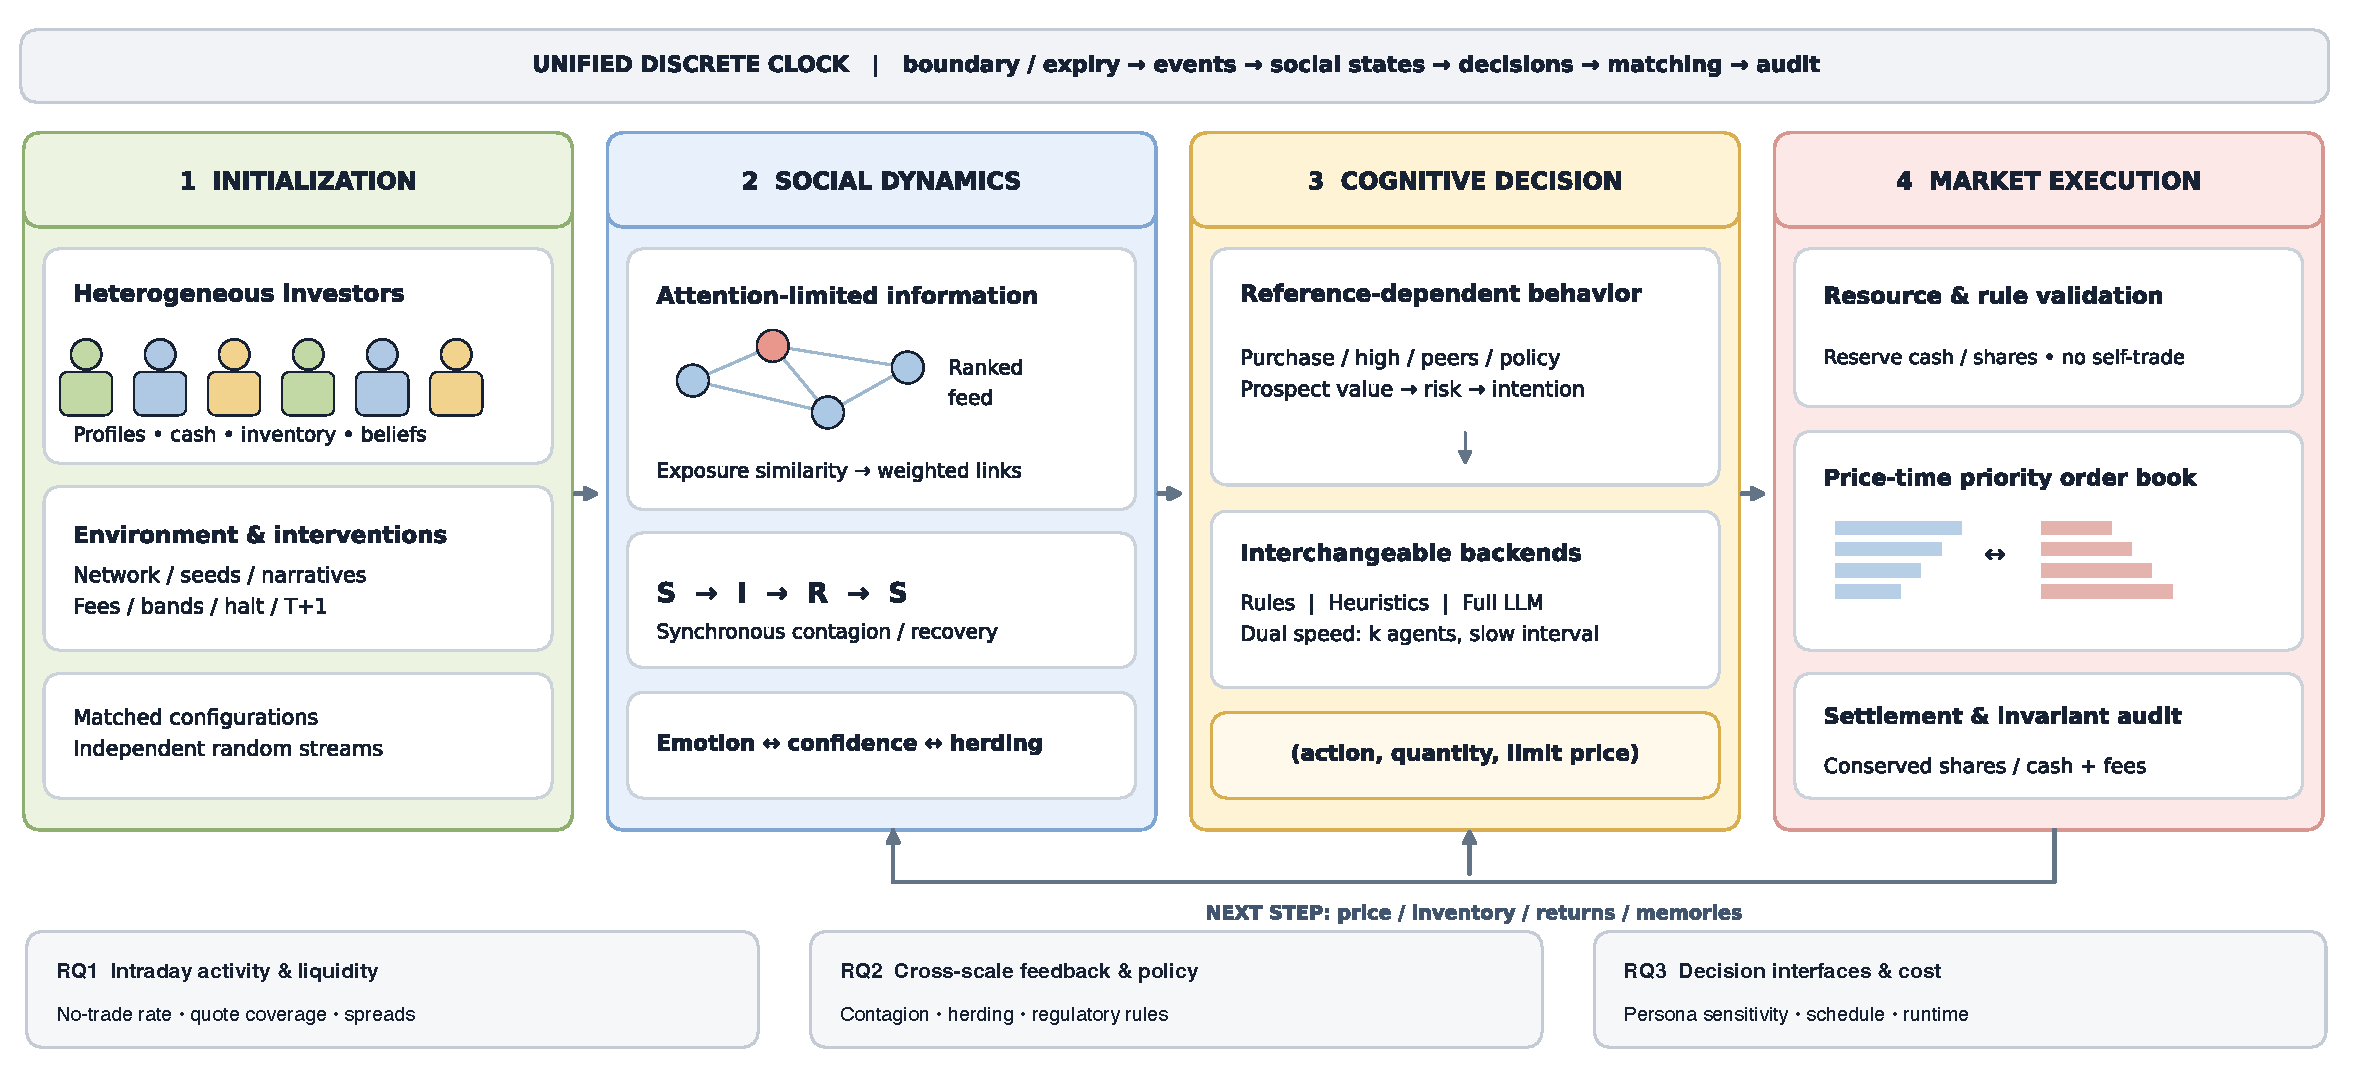
\includegraphics[width=\textwidth]{figures/fig1_methodology_overview.pdf}
  \caption{The Civitas Economica architecture. Portfolio exposures weight ties, group states shape orders, and settlement produces new prices and portfolios. Phases \ref{phase:boundary}--\ref{phase:events} prepare the market. Phases \ref{phase:social}--\ref{phase:behavior} update information and behavior using Equations~\eqref{eq:exposure}--\eqref{eq:confidence_update}. Phase \ref{phase:decision} produces orders through Equations~\eqref{eq:aggregate_v}--\eqref{eq:order_quantity} or the decision interface, which supports the cache in Equation~\eqref{eq:cache_signature}. Phases \ref{phase:execution}--\ref{phase:commit} process arrivals in seeded order, settle trades, and commit the ledger under Equations~\eqref{eq:settle_b}--\eqref{eq:invariants}.}
  \Description{Three economic relation scales linked by an eight-phase clock, from peer exposure and group states to orders, market settlement, and next-step feedback.}
  \label{fig:overview}
\end{figure*}

\subsection{Unified Discrete Clock and Causal Scheduling}
\label{sec:method:clock}

Each step separates updates visible to decision makers from the trades produced by their decisions.
\begin{enumerate}[leftmargin=*, label=(\arabic*), ref=\arabic*]
  \item\label{phase:boundary} \textbf{Trading Day Boundary.} The first day starts at $P_0$. At each subsequent day boundary, where $t>1$ and $(t-1)\bmod T_{\mathrm{day}}=0$, set $P^{\mathrm{base}}_t=P_{t-1}$ and release expired inventory locks. The daily band is $[P_t^{\mathrm{lower}},P_t^{\mathrm{upper}}]=[P^{\mathrm{base}}_t(1-L),P^{\mathrm{base}}_t(1+L)]$.
  \item\label{phase:expiry} \textbf{Order Expiration and Reservation Release.} Cancel expired orders and return remaining reserved cash and shares to available balances.
  \item\label{phase:events} \textbf{Exogenous Events and Public Narratives.} Publish scheduled macroeconomic announcements, earnings reports, or regulatory shocks.
  \item\label{phase:social} \textbf{Social Interaction and Message Filtering.} Update exposure-weighted edges, select messages under the attention budget, and advance the synchronous SIRS process from the post-event states.
  \item\label{phase:behavior} \textbf{Sentiment and Confidence.} Compute herding weights from lagged confidence and the pessimistic-neighbor share. Update sentiment $s_{i,t}$ using post-transition infection, lagged peer sentiment, and the previous return. Update confidence $q_{i,t}$ according to the herding trigger.
  \item\label{phase:decision} \textbf{Cognitive Decisions.} All agents update their reference prices. The activation mask $A^{\mathrm{act}}_{i,t}\sim\mathrm{Bernoulli}(p_{\mathrm{act}})$ is sampled across agents and steps and shared within matched comparisons. Active agents use their assigned backend to return \texttt{(action, quantity, price)}. Inactive agents submit \texttt{HOLD}.
  \item\label{phase:execution} \textbf{Validation, Matching, and Settlement.} Process intents in seeded arrival order, checking cash or sellable shares. Match admissible orders against the book by price and time priority, and settle fills and fees.
  \item\label{phase:commit} \textbf{Ledger Auditing and State Records.} Check cash and share conservation and record execution, ledger, and agent state.
\end{enumerate}

An agent sees the last committed price and book, its current available resources and psychological state, and events visible at the current step. Its own execution receipts become visible from step $t+1$. With a one-step order lifetime, remaining orders expire before new intents arrive, so the quoted depth in the observation is historical.

\subsection{Three Scales and Investor Archetypes}
\label{sec:method:population}

\paragraph{Person to Person.} Exposure similarity determines the weight of a peer relationship. Let $C_{i,t-1}$ and $Q_{i,t-1}$ be the cash and shares held by agent $i$ after step $t-1$. Prices and cash in the behavioral rules are in major currency units. Risk exposure is the fraction of wealth held in the risky asset.
\begin{equation}
x^{\mathrm{exp}}_{i,t-1}=\frac{Q_{i,t-1}P_{t-1}}{C_{i,t-1}+Q_{i,t-1}P_{t-1}+\epsilon}.
  \label{eq:exposure}
\end{equation}
Each edge moves toward a target set by the similarity of the two portfolios.
\begin{equation}
\begin{split}w_{ij,t}=\clip\bigl(&(1-\omega)w_{ij,t-1}\\&+\omega(2-|x_i^{\rm exp}-x_j^{\rm exp}|),w_{\min},w_{\max}\bigr).\end{split}
  \label{eq:edge_weight}
\end{equation}
Both exposures in the edge update are evaluated at step $t-1$. We use $\omega=0.1$ and $(w_{\min},w_{\max})=(1,2)$. Cash and price are expressed in the same currency unit, and $\epsilon>0$ defines exposure for zero wealth. A smaller exposure difference raises the target edge weight. These ties weight neighborhood aggregates. Equation~\eqref{eq:message_score} selects messages under limited attention.

\paragraph{Person to Group.} The selected feed and weighted neighborhood states drive infection, sentiment, and confidence in Equations~\eqref{eq:infection_prob}--\eqref{eq:confidence_update}. The nine archetypes have sampling probabilities of 70\% for retail traders, 8\% for mutual funds, 5\% for pension funds, 4\% for insurers, 4\% for proprietary desks, 4\% for market makers, 1\% for stabilization funds, 2\% for rumor-sensitive traders, and 2\% for arbitrageurs. Archetypes define role labels and the persona-specific decision parameters in Section~\ref{sec:method:cognition}. We sample them independently of the Watts--Strogatz network, so role and network position can vary separately~\cite{watts1998collective}. Baseline loss aversion is $2.25$ for all archetypes.

\paragraph{Group to Society.} This scale represents collective outcomes in the modeled market. Orders from all archetypes meet in the limit order book under common trading rules, producing transaction prices, volume, spreads, and depth. Settlement in Equations~\eqref{eq:settle_b}--\eqref{eq:invariants} changes portfolios. Prices and returns enter the next step's exposure, references, and sentiment. These updates close the feedback from market outcomes to individual decisions.

\subsection{Social Layer: Attention-Bounded Contagion and Confidence-Dependent Herding}
\label{sec:method:social}

\paragraph{Attention-Bounded Information Filtering.} Let $\mathcal N_i$ be agent $i$'s social neighborhood. In phase~(\ref{phase:social}), agent $i$ scores messages from neighbors in the infected state after the external event has been applied.
\begin{equation}
\begin{split}h_{ij,t}={}&\theta_1(1-|s_i-s_j|/2)+\theta_2\ind\{u_i=u_j\}\\&+\theta_3(1-|a_i-a_j|)+\theta_4 Inf_j+\theta_5 E_{ij,t-1}.\end{split}
  \label{eq:message_score}
\end{equation}
The terms measure sentiment similarity, shared topic, risk similarity, source influence, and past exposure. Sentiment and risk come from the previous committed step, and nonnegative weights sum to one. The highest-scoring messages form $\mathcal F_{i,t}$, with at most $A_i$ messages and ties broken by source identifier.

\paragraph{Synchronous SIRS Panic Propagation.} The model represents panic with Susceptible ($S$), Infected ($I$), and Recovered ($R$) states. Infection pressure combines the weighted infection share across the neighborhood with the messages selected by attention.
\begin{equation}
\begin{split}\rho_{i,t}&=\frac{\sum_j w_{ij,t}\ind\{\widetilde X_{j,t}=I\}}{\sum_jw_{ij,t}},\\p^{\rm inf}_{i,t}&=\clip\bigl(\overline{h_{ij,t}\mathrm{sim}_{ij,t}}_{\mathcal F_{i,t}}(\kappa_0+\kappa_1\rho_{i,t})\\&\hspace{5em}+\kappa_2\rho_{i,t},0,1\bigr).\end{split}
  \label{eq:infection_prob}
\end{equation}
Here $\widetilde X$ is the post-event, pre-transition state and $\mathrm{sim}_{ij,t}=1-|s_i-s_j|/2$ uses lagged sentiment. The sums in $\rho_{i,t}$ run over $\mathcal N_i$, and the overbar takes the arithmetic mean of $h_{ij,t}\mathrm{sim}_{ij,t}$ over $\mathcal F_{i,t}$. An empty feed has mean zero, and an isolated agent's infection share is zero. A susceptible agent becomes infected with probability $\clip(\beta p^{\rm inf}_{i,t}c_i,0,1)$, where $c_i$ is herding propensity.

Recovery depends on infection duration and the concentration of an agent's exposure.
\begin{equation}
p^{\rm rec}_{i,t}=\clip\bigl(\gamma(1+\eta_d\widetilde D_{i,t})(1-\eta_e e_{i,t}),0,1\bigr).
  \label{eq:recovery_prob}
\end{equation}
Exposure follows $E_{ij,t}=(1-\zeta_E)E_{ij,t-1}+\zeta_E\ind\{j\in\mathcal F_{i,t}\}$. Its concentration is $e_{i,t}=\sum_j(E_{ij,t}/\sum_kE_{ik,t})^2$, with zero concentration when total exposure is zero. The duration $\widetilde D$ is evaluated before the transition. A recovered agent becomes susceptible with probability $\clip(\delta(1+\eta_\psi p^{\rm inf}_{i,t}),0,1)$. Each transition is sampled from the post-event state. This makes the propagation update synchronous.

\paragraph{Confidence-Dependent Herding.} Continuous sentiment $s_{i,t}\in[-1,1]$ combines inertia, infection, peer sentiment, and the market return.
\begin{equation}
\begin{split}s_{i,t}=\clip\bigl(&(w_i^D-\Delta_{i,t})s_{i,t-1}-w_i^g\ind\{X_{i,t}=I\}\\&+(w_i^N+\Delta_{i,t})\bar s^N_{i,t-1}\\&+w_i^M\clip(r_{t-1}/r_*,-1,1)+\epsilon_s,-1,1\bigr).\end{split}
  \label{eq:sentiment_update}
\end{equation}
The peer term averages lagged sentiment with edge weights. An isolated agent uses its own lagged sentiment. The default return scale is $r_*=0.01$, and $\epsilon_s\sim\mathcal N(0,\sigma_s^2)$ with $\sigma_s=0.02$. Herding transfers weight from the agent's own prior sentiment to that of peers, preserving their combined weight~\cite{deutsch1955study}.
\begin{equation}
\Delta_{i,t}=H_{i,t}\eta_H(1-q_{i,t-1})w_i^D,\qquad H_{i,t}=\ind\{b^N_{i,t}>0.5\}.
  \label{eq:herding_shift}
\end{equation}
Here $b^N_{i,t}$ is the edge-weighted fraction of neighbors with sentiment below $-s_*$. Confidence decreases when the trigger fires and otherwise returns toward $q_0$. The herding ablation sets $\eta_H=\eta_q=0$ and retains the recovery term.
\begin{equation}
\begin{split}q_{i,t}=\clip\bigl(&q_{i,t-1}-H_{i,t}\eta_q(1-q_{i,t-1})\\&+(1-H_{i,t})\eta_{\rm rec}(q_0-q_{i,t-1}),0,1\bigr).\end{split}
  \label{eq:confidence_update}
\end{equation}


\subsection{Behavioral Core: Multi-Reference Prospect Theory and Order Generation}
\label{sec:method:behavior}

\paragraph{Four Adaptive Reference Prices.} After the social update, agents update four anchors in phase~(\ref{phase:decision}) for acquisition cost ($R^p$), the rolling local high ($R^h$), peer consensus ($R^n$), and the policy signal ($R^e$).
\begin{align}
 R^p_{i,t}&=(1-\kappa_p)R^p_{i,t-1}+\kappa_p T^p_{i,t},\label{eq:ref_p}\\
 R^h_{i,t}&=(1-\kappa_h)R^h_{i,t-1}+\kappa_h \max_{v=\max(0,t-H_h)}^{t-1}P_v,\label{eq:ref_h}\\
 R^n_{i,t}&=(1-\kappa_n)R^n_{i,t-1}+\kappa_nP_{t-1}(1+\xi_n\bar s^N_{i,t-1}),\label{eq:ref_n}\\
 R^e_{i,t}&=(1-\kappa_e)R^e_{i,t-1}+\kappa_eP_{t-1}(1+\xi_e u_t^{\rm policy}).\label{eq:ref_e}
\end{align}
For a nonempty position the cost target is $T^p=K$, where $K$ is the position cost basis excluding fees. An empty position uses $T^p=P_{t-1}$. A policy state persists until a subsequent event changes it. Event text is visible at release.

\paragraph{Prospect Valuation and Loss Pressure.} An asymmetric power function maps reference deviations to prospect value~\cite{tversky1992advances}.
\begin{equation}
v_i(z)=\begin{cases}z^\alpha&z\ge0,\\-\lambda_i(-z)^\alpha&z<0.\end{cases}
  \label{eq:prospect_v}
\end{equation}
In the full model, $\lambda_i>1$ sets loss aversion and $\alpha\in(0,1)$ sets diminishing sensitivity. We define signed deviations from the cost and price high using the reference as the denominator. For peer and policy anchors we use the latest price as denominator and reverse the sign convention. The weighted sum enters the value function once.
\begin{equation}
\begin{split}x^\bullet_{i,t}&=\begin{cases}(P_{t-1}-R^\bullet_{i,t})/R^\bullet_{i,t}&\bullet=p,h,\\(R^\bullet_{i,t}-P_{t-1})/P_{t-1}&\bullet=n,e,\end{cases}\\z_{i,t}&=\sum_\bullet\omega_\bullet x^\bullet_{i,t},\quad V_{i,t}=v_i(z_{i,t}),\quad d_{i,t}=\tanh(\kappa_vV_{i,t}).\end{split}
  \label{eq:aggregate_v}
\end{equation}
The retrospective loss fraction $b_{i,t}=(\omega_p\mathbf{1}\{P_{t-1}<R^p_{i,t}\}+\omega_h\mathbf{1}\{P_{t-1}<R^h_{i,t}\})/(\omega_p+\omega_h)$ weights the cost and high-price references above the current price and enters the bounded loss-pressure function.
\begin{equation}
  \ell_{i,t} = \clip\left( \lambda_i (1 + \chi b_{i,t}), \ell_{\min}, \ell_{\max} \right).
  \label{eq:loss_pressure}
\end{equation}
Current risk tolerance $a_{i,t}\in[0,1]$ combines confidence, lagged risk tolerance, sentiment, valuation direction, and loss pressure.
\begin{equation}
\begin{split}a_{i,t}=\clip\bigl(&\omega_a^q q_{i,t}+\omega_a^a a_{i,t-1}+\omega_a^s s_{i,t}\\&+\omega_a^d d_{i,t}-\omega_a^\ell\max(0,(\ell_{i,t}-1)/\nu),0,1\bigr).\end{split}
  \label{eq:risk_tolerance}
\end{equation}

\paragraph{Trading Intention and Limit Orders.} Valuation direction, sentiment, and risk tolerance determine the intention score $\tau_{i,t}\in[-1,1]$.
\begin{equation}
\tau_{i,t}=\clip\bigl(\omega_\tau^d d_{i,t}+\omega_\tau^s s_{i,t}+\omega_\tau^a(a_{i,t}-0.5),-1,1\bigr).
  \label{eq:intent_score}
\end{equation}
At threshold $\delta_a\ge0$, the agent draws a buy, sell, or hold action using the following probabilities.
\begin{equation}
\begin{split}p_i^b&=\sigma(\kappa_a(\tau_{i,t}-\delta_a)),\\p_i^s&=\sigma(-\kappa_a(\tau_{i,t}+\delta_a)),\qquad p_i^h=1-p_i^b-p_i^s.\end{split}
  \label{eq:action_selection}
\end{equation}
An independent $U_i\sim U(0,1)$ scales the order size. The buy fraction is $f_i^b=U_i[f_{\min}+(f_{\max}-f_{\min})a_i]$. The sell fraction is $f_i^s=U_i[f_{\min}+(f_{\max}-f_{\min})\max(-\tau_i,0)]$. Rule baselines share the mean-corrected lognormal quote perturbations, drawn independently of action direction.
\begin{equation}
\begin{split}\widetilde p_i&=P_{t-1}\exp(\epsilon_p-\sigma_p^2/2),\\p_i^{\rm lim}&=\Delta_p\max\{1,\operatorname{round}_{\rm even}(\widetilde p_i/\Delta_p)\}.\end{split}
  \label{eq:limit_price}
\end{equation}
Here $\epsilon_p\sim\mathcal N(0,\sigma_p^2)$. At a rounding tie, the quote rounds to an even tick. The exchange rejects orders outside the daily price band. Quantities are integers bounded by available resources.
\begin{equation}
  n_i = \begin{cases}
    \bigl\lfloor f^b_{i,t} C_{i,t}^{\mathrm{free}} / \bigl(p_i^{\mathrm{lim}}(1+c)\bigr) \bigr\rfloor & \mathrm{BUY}, \\
    \bigl\lfloor f^s_{i,t} Q_{i,t}^{\mathrm{free}} \bigr\rfloor & \mathrm{SELL}.
  \end{cases}
  \label{eq:order_quantity}
\end{equation}
Here $c$ is the commission rate. Zero quantities become \texttt{HOLD}.

\subsection{Microstructure, Limit Order Book, and Ledger Invariants}
\label{sec:method:microstructure}

\paragraph{Escrow Reservation and Price--Time Priority.} Buy orders reserve cash for limit-price notional and buyer commission. Sell orders reserve sellable shares. The ledger tracks these reservations within each account. The ledger stores $10^6$ integer micro-units per major currency unit: $C_{i,t}^{\rm minor}=10^6 C_{i,t}$. Fill notionals and fees use the same micro-unit scale. For integer fill notional $V$, each side pays commission $f_c=\lfloor cV\rfloor$ and the seller pays tax $f_\tau=\lfloor\tau^{\rm tax}V\rfloor$.

Bids are ordered by descending price and asks by ascending price, with earlier orders first at each price. Crossing orders match at the resting price. A fill of $q^*$ shares updates the buyer $b$, seller $s$, and the fee account $F^{\rm minor}$ as follows.
\begin{align}
  C_b^{\rm minor} &\gets C_b^{\rm minor} - V-f_c, \quad Q_b \gets Q_b + q^*, \label{eq:settle_b} \\
  C_s^{\rm minor} &\gets C_s^{\rm minor} + V-f_c-f_\tau, \quad Q_s \gets Q_s - q^*, \label{eq:settle_s} \\
  F^{\rm minor} &\gets F^{\rm minor} +2f_c+f_\tau. \label{eq:settle_fees}
\end{align}
A fill releases excess escrow for the executed quantity. Resources for any unfilled quantity remain reserved until execution, cancellation, or expiration.

\paragraph{Ledger Conservation.} Reserved resources remain part of account balances. At every commit, the engine audits total cash across the agent and fee accounts and total shares across agents.
\begin{equation}
\begin{aligned}
 \sum_i C_{i,t}^{\rm minor}+F_t^{\rm minor}&=\sum_i C_{i,0}^{\rm minor}+F_0^{\rm minor},\\
 \sum_{i=1}^N Q_{i,t}&=\sum_{i=1}^N Q_{i,0}.
\end{aligned}
  \label{eq:invariants}
\end{equation}
Any nonzero residual triggers an audit error.

\subsection{Cognitive Architectures and Dual-Speed Scheduling}
\label{sec:method:cognition}

All four backends share information eligibility and return \texttt{(action, quantity, price)}. The same execution kernel validates and matches their orders.
\begin{enumerate}[leftmargin=*, label=(\arabic*)]
  \item \textbf{Numerical Rules (System 1).} Evaluate Equations~(\ref{eq:exposure})--(\ref{eq:order_quantity}) as the rule baseline.
  \item \textbf{Persona Heuristics.} Adjust a target portfolio exposure for valuation, trend, and sentiment. An archetype-specific band and a resource cap govern the resulting order.
  \item \textbf{Full LLM Agents (System 2).} Serialize the agent's profile, account state, market facts, and eligible records. Validate response identity and intent type, and check that \texttt{evidence\_ids} are unique members of the visible ID set (Appendix~\ref{app:prompt}). The exchange checks price bands and available resources at execution.
  \item \textbf{Dual-Speed Hybrid Scheduling.} All agents perform lightweight System 1 updates. A fixed set of $k$ agents sampled by persona requests System 2 responses when active and $t\bmod T_{\mathrm{slow}}=0$.
\end{enumerate}

The market runner admits rule decisions and both synthetic and archived model responses. Live model requests use the same decision contract in a separate fixed-observation harness.

\paragraph{Resource-Aware Strategy Caching.} At a System 2 request step, the scheduler caches a normalized direction and resource commitment so later orders can adapt to current prices and balances.
\begin{equation}
\begin{aligned}
 \widehat d_i &=
 \begin{cases}
   +1 & \mathrm{BUY}, \\
   -1 & \mathrm{SELL}, \\
   0 & \mathrm{HOLD},
 \end{cases} \\
 \widehat f_i &=
 \begin{cases}
   \min\!\bigl(1,n_i/M_i^{\mathrm{action}}\bigr) & M_i^{\mathrm{action}}>0, \\
   0 & \text{otherwise.}
 \end{cases}
\end{aligned}
  \label{eq:cache_signature}
\end{equation}
Here $M_i^{\mathrm{action}}$ is conservative capacity at the requested limit price under a continuous commission budget bound. A \texttt{HOLD} decision has zero resource commitment. When reusing the cache, an active agent keeps $\widehat d_i$ and $\widehat f_i$, recomputes a limit price around $P_{t'-1}$ with the shared quote perturbation, and floors the committed fraction of current capacity to obtain an integer quantity. Reuse is allowed for ages $1$ through $A_{\max}$, inclusive. A missing or expired entry invokes the rule policy. A recognized response failure clears the cache and returns \texttt{HOLD}. A reused intent with zero final quantity returns \texttt{HOLD}.

\paragraph{Scheduled Model Request Budget.} Over $T$ steps, full LLM scheduling offers $p_{\mathrm{act}}NT$ expected request opportunities and dual-speed scheduling offers $p_{\mathrm{act}}k\lfloor T/T_{\mathrm{slow}}\rfloor$. Their ratio is approximately
\begin{equation}
  \text{Request ratio} \approx \frac{k}{N \cdot T_{\mathrm{slow}}}.
  \label{eq:cost_ratio}
\end{equation}
For $N=100$, $k=10$, and $T_{\rm slow}=10$, a horizon divisible by $T_{\rm slow}$ yields 99\% fewer expected request opportunities. Actual cost also depends on response usage and execution time.
\paragraph{Analysis Tools.} We used OpenAI Codex to assist with implementation cross-checks, analysis of archived records, and manuscript editing. We checked the reported values against the archived data.

\section{Experimental Evaluation}
\label{sec:experiments}

\subsection{Benchmarks and Execution Checks}
\label{sec:setup}

The benchmarks in Table~\ref{tab:measured_design} work backward from observed prices. The intraday runs (RQ1) measure when trades occur and both sides of the book are present under matched randomness. The shared-parent branches (RQ2) then track how a common infection event changes social states and how behavioral and regulatory interventions affect orders and fills. The fixed-observation and schedule benchmarks (RQ3) move upstream to compare intents across decision backends and identify which scheduled requests could carry a public announcement. Rule-world profiles measure the cost of retaining and verifying the state history that makes these paths auditable.

\begin{table*}[t]
  \centering\small
  \caption{\tr{实测基准及离线调度核对的配置。长周期参考配置见附录~\ref{app:benchmark_details_zh}。}{Settings for the Measured Benchmarks and Offline Schedule Audit. Appendix~\ref{app:benchmark_details} gives the prospective long-horizon configuration.}}
  \label{tab:measured_design}
  \begin{tabularx}{\textwidth}{@{}p{0.24\textwidth} p{0.28\textwidth} X@{}}
    \toprule
    \tr{评估任务}{Evaluation} & \tr{执行配置}{Settings} & \tr{比较单位}{Unit of comparison} \\
    \midrule
    \tr{日内交易活动（RQ1）}{Intraday activity (RQ1)} &
    $N=100$, $T=T_{\rm day}=100$, $p_{\rm act}=0.05$ &
    \tr{三个匹配种子，各比较三种规则策略。}{Three matched seeds, each shared by three rule policies.} \\
    \tr{共同父世界分支（RQ2）}{Shared-parent branches (RQ2)} &
    $N=20$, $T_{\rm day}=4$, $p_{\rm act}=1$, \tr{27 步事件窗}{27 event steps} &
    \tr{一个父世界，十一条分支。}{Eleven branches from one parent world.} \\
    \tr{固定观察（RQ3）}{Fixed observations (RQ3)} &
    \tr{九类画像 $\times$ 三类对比 $\times$ 两个状态}{Nine archetypes $\times$ three contrasts $\times$ two states} &
    \tr{54 次真实 LLM 请求，构成 27 对比较。}{54 live LLM requests, organized into 27 pairs.} \\
    \tr{离线调度核对（RQ3）}{Offline scheduling (RQ3)} &
    $N=100$, $p_{\rm act}=0.05$, $k=10$, $T_{\rm slow}=10$ &
    \tr{20 个固定种子在公告发布步的计划资格。}{Scheduled eligibility at announcement release across 20 fixed seeds.} \\
    \tr{规则运行剖面（RQ3）}{Rule profiles (RQ3)} &
    \tr{同一平台 $N=100$、$T=100,200$；另一平台 $N=1{,}000$、$T=12$}{Same host $N=100$, $T=100,200$; second host $N=1{,}000$, $T=12$} &
    \tr{Mac 各期限一次完整剖面；ASUS 保存 12 步、终期剖面未完成。}{One complete Mac profile per horizon. The ASUS run saved 12 steps and stopped during final profiling.} \\
    \bottomrule
  \end{tabularx}
\end{table*}


The three rule policies use seeds 932201--932203. Across all 900 committed steps, the cash, share, and fee residuals are zero. Read-only restoration on the same platform matches the terminal state hash in all nine trajectories (Table~\ref{tab:invariants}). Each seed is the unit of comparison across policies.

\subsection{Market Activity and Quote Coverage (RQ1)}
\label{sec:exp:rq1}

We hold the activity mask, lognormal quote shocks, resource constraints, and matching rules fixed within each seed. Zero-intelligence agents draw buy and sell actions with symmetric probabilities and can hold~\cite{gode1993allocative}. The homogeneous linear-value policy retains acquisition cost and the recent high as anchors. Its valuation is linear, its risk tolerance is fixed at 0.5, and its order policy excludes social and loss feedback.

\begin{figure*}[t]
 \centering
 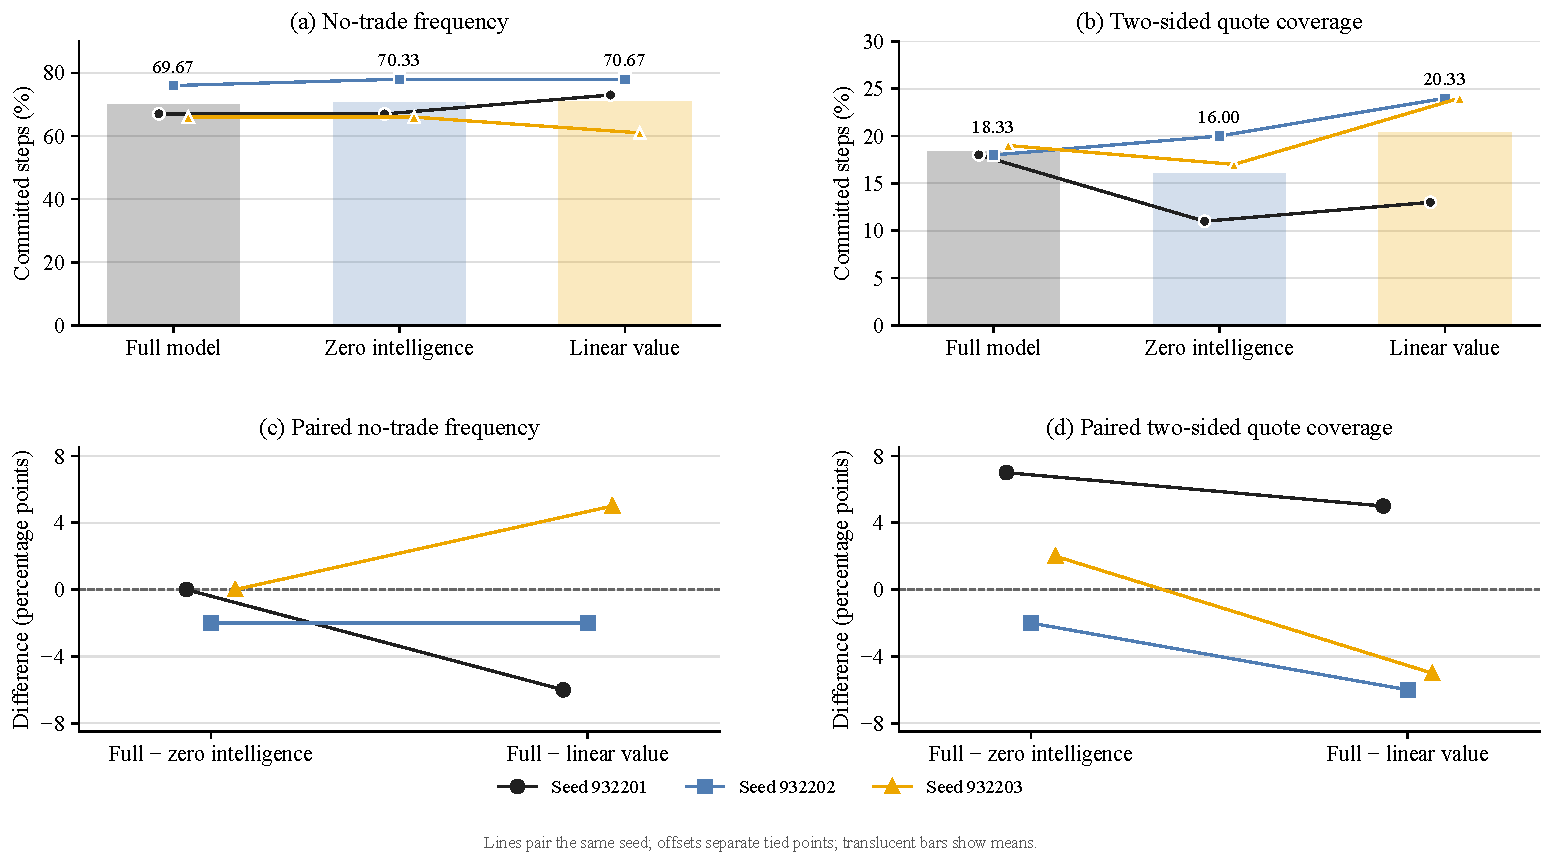
\includegraphics[width=0.96\textwidth]{figures/fig2_rq1_stylized_facts.pdf}
 \caption{Intraday activity in nine rule trajectories. The upper panels show the percentage of steps without trades and the percentage with two-sided quotes. The lower panels show the full model minus each baseline within the same seed, in percentage points. Bars in the upper panels denote means, with matched trajectories linked across policies. Small horizontal offsets distinguish overlapping markers.}
 \Description{Two panels of activity and quote coverage by policy and two panels of matched-seed differences.}
 \label{fig:rq1}
\end{figure*}

\paragraph{Quote coverage varies across matched seeds.}
With an activation probability of 0.05 and a one-step order lifetime, 61--78\% of steps have no fills and 11--24\% have quotes on both sides. The full model averages 69.67\% of steps without trades and 18.33\% with two-sided quotes. The corresponding figures are 70.33\% and 16.00\% for zero intelligence and 70.67\% and 20.33\% for linear value. The full-minus-baseline coverage differences are $+7,-2,+2$ percentage points against zero intelligence and $+5,-6,-5$ against linear value. The ranking changes across the three blocks (Figure~\ref{fig:rq1}, Table~\ref{tab:rq1_results}).

The quoted spread $10^4(P^{\rm ask}-P^{\rm bid})/P^{\rm mid}$ is conditional on both queues being present at a tradable step. Reporting quote coverage alongside the spread makes its sampling denominator explicit. Each trajectory spans one model trading day. The corresponding multi-day protocol uses daily log returns $r_d=\log(P_d/P_{d-1})$ to evaluate excess kurtosis, return and absolute-return autocorrelations, and the correlation of volume with $|r_d|$~\cite{cont2001empirical} (Appendix~\ref{app:benchmark_details}).

\subsection{Feedback Across Scales (RQ2)}
\label{sec:exp:rq2}

\begin{figure*}[t]
 \centering
 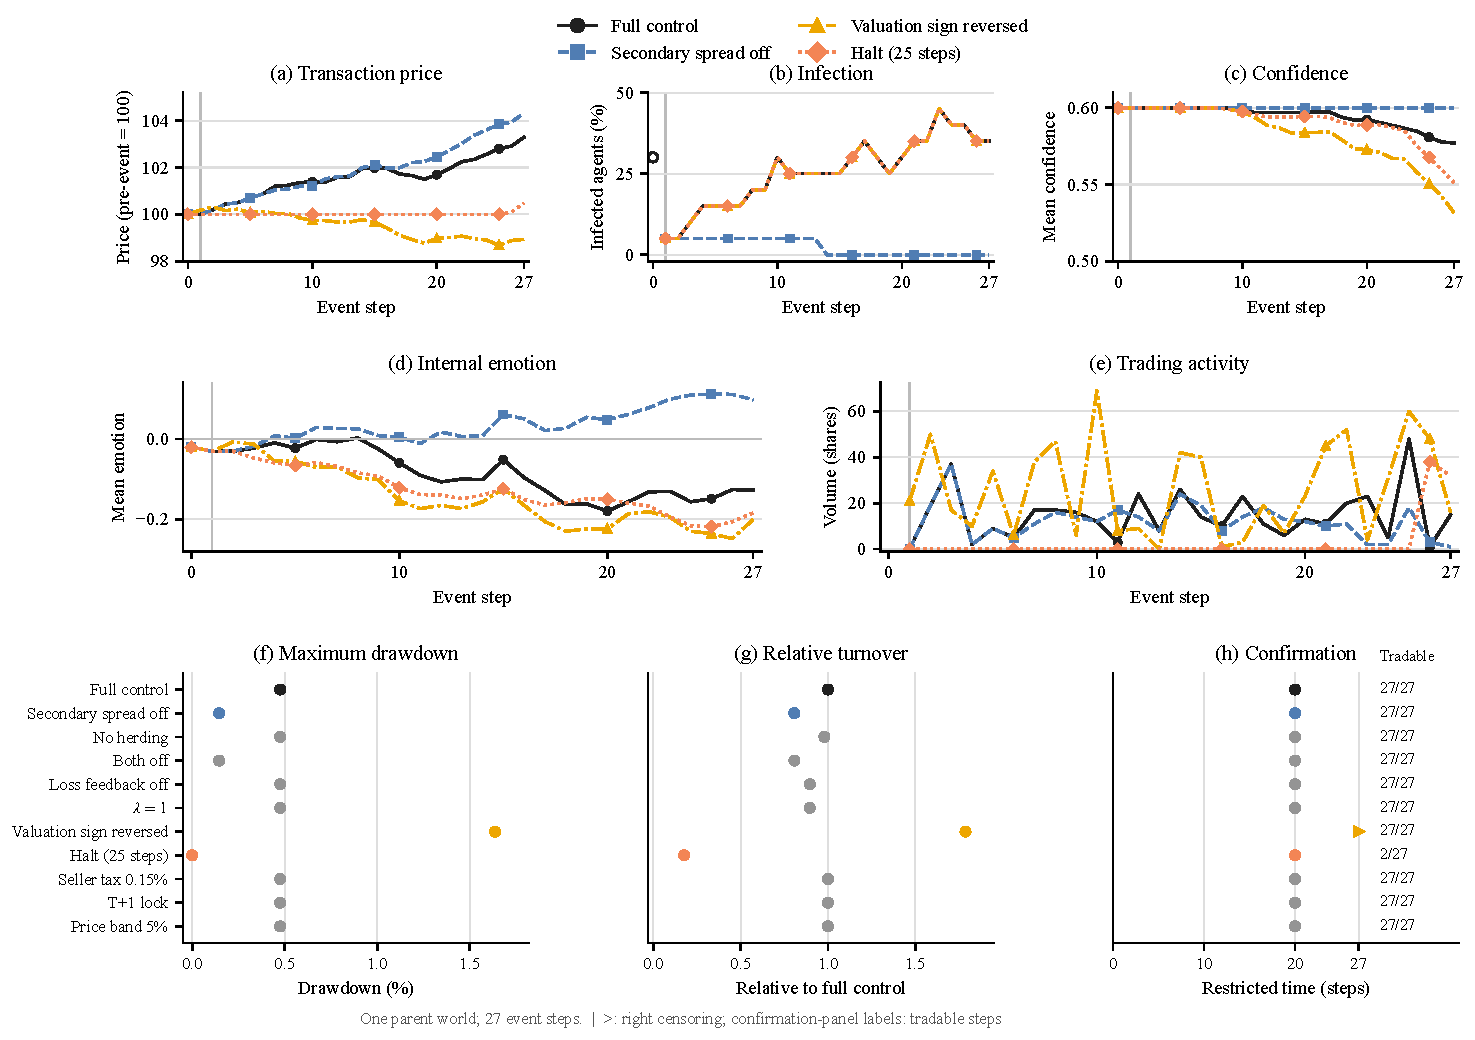
\includegraphics[width=\textwidth]{figures/fig3_rq2_mechanisms_policy.pdf}
 \caption{Social, behavioral, and market responses in one shared parent world. The time-series panels align infection, population means of model confidence and sentiment, indexed price, and share volume on the same event clock. The open marker in panel (b) denotes the pre-event checkpoint (6 of 20 infected). At $u=1$, the common event resets all SIRS states to susceptible and seeds one infection (1 of 20). The outcomes below show all eleven branches. The arrowhead marks right censoring at $u=27$.}
 \Description{Five aligned event-time series and three outcome plots for drawdown, turnover, and price confirmation.}
 \label{fig:rq2}
\end{figure*}

\paragraph{Shared-checkpoint design.}
All branches begin at the fifth commit of seed 933001, with 20 investors, four steps per day, and every investor active at each event step. Six investors are already infected at the common checkpoint $u=0$. At $u=1$ (tick 6), the event sets all investors to susceptible and directly infects one investor. The 30\% checkpoint prevalence and the 5\% prevalence at the first event commit therefore describe the states before and after this common reinitialization. The branches share the random streams for 27 event steps. We record infection, population mean confidence and sentiment, the last-trade price, and traded share volume at each commit (Figure~\ref{fig:rq2}).

Maximum drawdown is the largest decline from a running peak initialized at the pre-event price. Relative turnover divides each branch's traded share volume by that of the full control. The price-confirmation rule records the step completing 20 consecutive prices at or above 98\% of the pre-event price after the first global trough, which can be $u=0$. Unconfirmed times are right-censored at the window boundary (Table~\ref{tab:rq2_results}).

\paragraph{Social dynamics and market responses.}
In the full control, infection peaks at 45\% at $u=23$ (Figure~\ref{fig:rq2}b). Mean confidence begins to fall at $u=10$ and reaches 0.577 at the end of the window. Mean internal emotion reaches $-0.180$ at $u=20$ (panels c--d). Suppressing secondary contagion confines infection to the seeded investor until it clears at $u=14$. In that branch, confidence stays near 0.600 and mean emotion reaches $+0.112$ at $u=25$. Suppressing spread also reduces volume from 395 to 319 shares (panel e) and raises the final price index from 103.28 to 104.31 (panel a). Maximum drawdown falls from 0.4754\% to 0.1453\%, a reduction of 0.3301 percentage points (69.4\% relative).

Disabling confidence-dependent herding leaves peak infection at 45\%. Prices in the two branches coincide through $u=22$, including the local peak at $u=15$ and trough at $u=19$ that determine the 0.4754\% maximum drawdown. Volume already differs by one share at that trough, and total volume falls from 395 to 387 shares (relative turnover 0.9797). With $Y$ denoting drawdown and binary indices denoting contagion and herding, the four-branch interaction $Y_{11}-Y_{10}-Y_{01}+Y_{00}$ is zero in this world.

\paragraph{The sign of retrospective valuation changes the price response.}
The infection event changes the social state, and prices respond to the resulting orders and fills. In Equation~\eqref{eq:aggregate_v}, a price above a retrospective reference adds a positive term to the valuation and can raise the buying propensity when the other inputs are held fixed. The aggregate order direction also depends on the remaining references, sentiment, and risk. Reversing the retrospective signs lowers the final price to 1.07\% below the pre-event price, raises maximum drawdown to 1.6372\%, and raises relative turnover to 1.7873. The branch with $\lambda=1$ and the branch that also removes dynamic loss feedback both record 0.4759\% drawdown and 0.8962 relative turnover.

\paragraph{Trading rules affect different parts of the exchange.}
A 25-step halt leaves two tradable steps and a relative turnover of 0.1772. Drawdown is zero. The book is cleared at the start of the halt. The price carries forward for 25 steps with zero fills. During that interval, infection peaks at 45\%, and mean internal emotion reaches $-0.218$ at $u=25$. At $u=26$, 38 shares trade as matching resumes (Figure~\ref{fig:rq2}a--e). The other three policy branches retain all 27 tradable steps and produce the same 87 fills as the control. In the 5\% band branch, submitted and executed prices deviate at most 1.092\% from their contemporaneous daily anchors. The $T+1$ rule locks up to 72 shares and leaves the realized sell orders and fills unchanged. The 0.15\% seller tax changes the settlement debit directly, leaving share sizing in Equation~\eqref{eq:order_quantity} unchanged at a given state. In this window the tax receipts rise from 20.286250 to 60.858750 currency units, with the same fills.

\paragraph{The confirmation floor reflects the short event window.}
The first trough is the pre-event price in ten branches, all of which reach the earliest confirmation at step 20. The halted branch reaches that threshold using carried-forward prices during the suspension. The reversed-valuation branch reaches its first trough at step 25 and has two subsequent observations, leaving its time right-censored at 27. The series remain above the 98\% threshold throughout this parent-world comparison. Here the confirmation measure records elapsed observations after the trough. Tradable steps and turnover give it an economic interpretation.

\subsection{Decision Interfaces and Computational Cost (RQ3)}
\label{sec:exp:rq3}

\begin{figure*}[t]
 \centering
 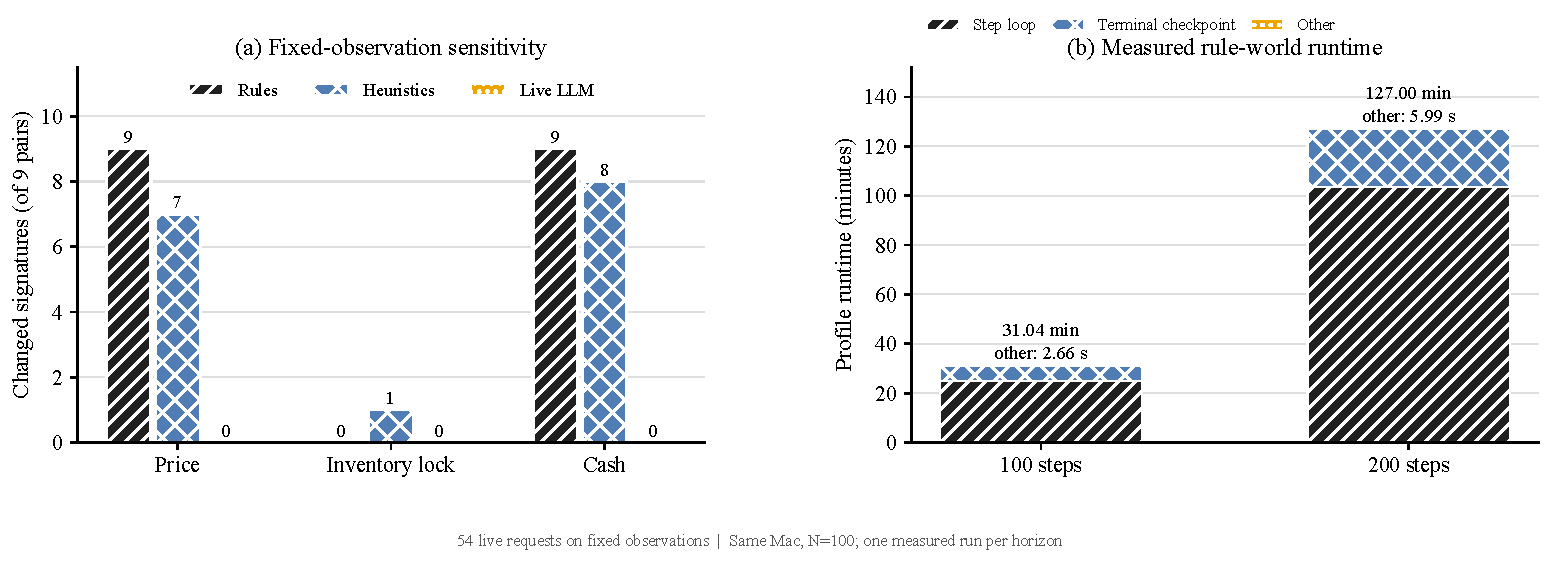
\includegraphics[width=\textwidth]{figures/fig4_rq3_cognition_cost.pdf}
 \caption{Fixed-observation responses and rule-world runtime. The response panel counts changes in economic action signatures across nine pairs per contrast. The runtime panel separates the durable step loop, terminal checkpoint, and remaining profile time for two $N=100$ runs on the same machine.}
 \Description{Action changes for price, inventory lock, and cash contrasts, and stacked profile times at two horizons.}
 \label{fig:rq3}
\end{figure*}

\paragraph{The fixed-observation benchmark exercises the decision contract.}
Nine archetypes, three contrasts (price, locked inventory, cash), and two states per contrast give 54 request cells, 45 distinct constructed observations, and 27 pairs. We use neutral wording, temperature zero, and a 2,048-token output limit. The request configuration and archived OpenAI API responses identify the model by the alias \texttt{gpt-6-luna}.

An economic action signature records direction, signed share quantity, and limit price. It changes in 18/27 rule pairs, 16/27 heuristic pairs, and 0/27 LLM pairs (Figure~\ref{fig:rq3}a and Table~\ref{tab:pilot}). Rules return 45 buys and nine holds. The LLM requests serialize both the constructed current state and the template behavioral trace stored in the private \texttt{behavior} field. The risk and price-reference values differ between these records in all 54 requests. Every model response is \texttt{HOLD} and passes the schema, protocol identity, evidence-ID, and resource checks. The evidence-ID check verifies that cited IDs are distinct members of the visible set. The signature contrast characterizes the backends on these constructed inputs. An additional comparison with aligned state and trace fields would be needed to isolate the effect of the discrepancy.

\paragraph{Archetype-specific order changes.}
Under numerical rules, the price contrast changes signed quantity by $-2$ shares for every archetype, and the cash contrast changes it by $-12$ shares (Figure~\ref{fig:persona_deltas}). Under persona heuristics, the price contrast shifts the arbitrageur and stabilization fund by $-102$ and $-63$ shares, respectively. The insurer changes from a 10-share sell order to \texttt{HOLD} in the inventory-lock contrast. In the separate price contrast, the insurer retains the same signed quantity and raises its limit by 1,002 ticks, the dagger-marked cell.

\begin{figure*}[t]
 \centering
 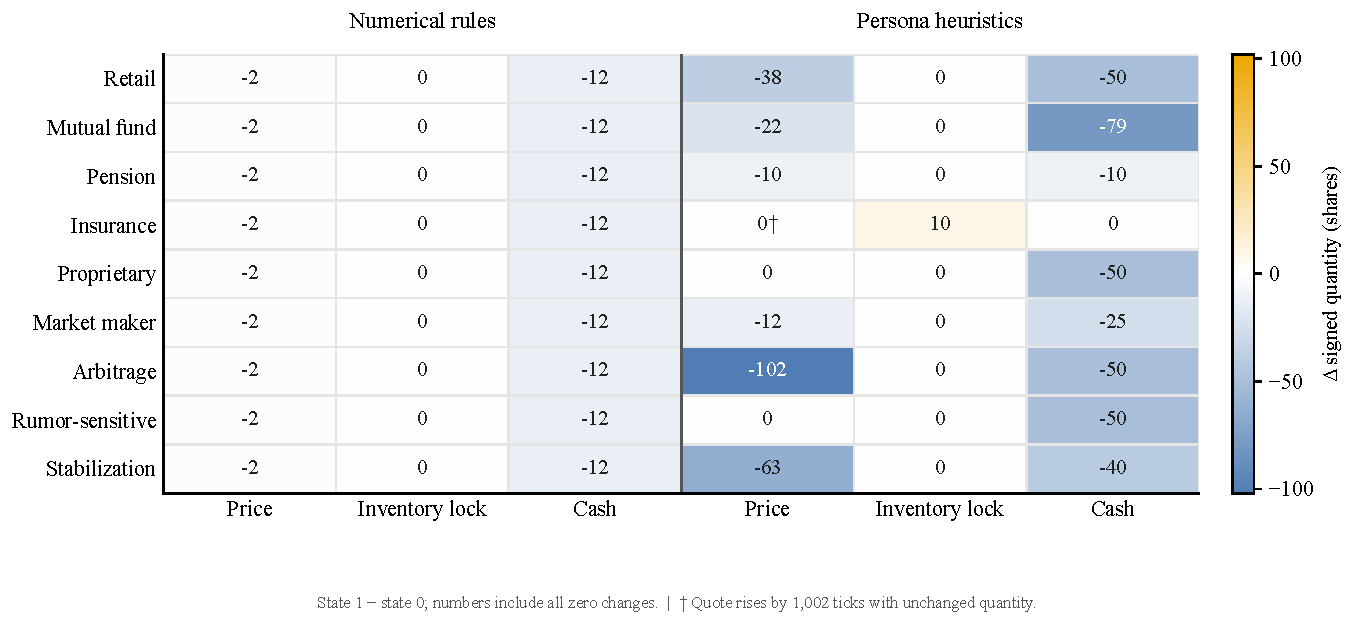
\includegraphics[width=0.96\textwidth]{figures/archetype_order_response.pdf}
 \caption{Changes in signed order size across nine archetypes. Each cell gives the perturbed minus baseline share quantity for one contrast and backend. A buy has positive sign, a sell negative sign, and a hold zero quantity. A dagger marks a price change with unchanged quantity.}
 \Description{Nine rows of archetypes and six columns of signed order size changes for the rule and heuristic backends.}
 \label{fig:persona_deltas}
\end{figure*}

\paragraph{Request accounting and scheduled event access.}
The live batch uses 119,637 input and 9,306 output tokens in 69.597 seconds. Median request latency is 2.297 seconds. Logged usage and frozen rates give an accounted cost upper bound of USD 0.03456225 (Table~\ref{tab:rq3_results}). An offline check separately intersects the activation masks and request schedules at the announcement step. For 20 fixed seeds, the announcement coincides with a periodic request step. Full scheduling offers 101 eligible requests across all seeds. The periodic slow group offers one request in each of ten seeds. In the other ten, no slow-group agent is active at release (right panel of Figure~\ref{fig:schedule_exposure}). Equation~\eqref{eq:cost_ratio} gives the expected request fraction across a full horizon. The release-step counts show how the same schedule affects access to a specific announcement.

\paragraph{Cumulative recording drives a term in the runtime cost.}
Extending the same-seed, 100-agent rule world from 100 to 200 steps on an Apple M5 (24 GiB) increases the profiled time from 1,862.397 to 7,619.767 seconds, a factor of 4.091. Peak process memory increases from 1.239 to 2.486 GiB. The terminal checkpoint, which includes reconstruction from persisted deltas, takes 364.780 and 1,394.507 seconds. Execution, commit, durable publication, and the terminal checkpoint together account for 89.9\% and 91.0\% of the two profiles. The decision phase takes 2.895 and 5.789 seconds.

The archival implementation repeatedly validates, copies, and hashes growing histories of decisions, receipts, and ledger entries. When retained history grows linearly in $t$, a full scan per step contributes $\sum_{t=1}^{T}\mathcal{O}(t)=\mathcal{O}(T^2)$ at fixed population. This term describes the work of processing cumulative history. Figure~\ref{fig:rq3} shows the two measured profiles of the full runner. On the AMD Ryzen AI 7 H 350 platform, the 1,000-agent run saves all 12 steps and reaches a sampled memory peak of 1.692 GiB before the controller stops during final profiling. In three timing repeats of the same 100-agent, 12-step world, scalar-optimized strict validation reduces total time by 1.52--3.08\% (Figure~\ref{fig:timing_supp}).

\section{Discussion}
\label{sec:discussion}

\subsection{How social states reach the market}

Market feedback begins with differences in portfolios and information exposure. Common risk exposure increases the weight of an investor's existing ties. Once the investor receives a message, its effect depends on the local infection state and on how confidence changes the relative weights on personal and peer signals. These states shape an order before it meets other orders in the auction. Settlement then changes the portfolios and reference prices available at the next observation. The shared-parent comparison makes this sequence observable in the same market history up to the intervention.

Contagion and herding affect different margins in that comparison. Suppressing onward infection reduces the interim drawdown despite the upward drift of both price paths. Disabling herding changes the quantity traded at the trough of the same drawdown. The price and fill records therefore reveal a change in trading activity even before the price paths diverge. Reversing the retrospective valuation signs moves the price path below its starting point. Joint records of infection, confidence, and trades let a researcher distinguish these responses to mechanism switches. The effects are conditional on the parent state and the specified event.

\subsection{Trading institutions shape market access}

RQ1 uses two-sided coverage to identify the trading conditions under which a spread is observable. The halt in RQ2 makes the same point about transaction prices. During the halt, the carried-forward price records zero drawdown and satisfies the confirmation rule at step 20. Infection and sentiment continue to evolve during those same steps. Price-based assessments of recovery therefore need the contemporaneous trading opportunities and the social state. The other branches illustrate interventions at three distinct points. The price band tests admissible quotes, the settlement lock changes available inventory, and the tax redistributes cash at execution. In this history the submitted prices stay inside the band, and the additional restriction on shares leaves the submitted sell orders unchanged. The tax changes ledger balances with the same fills. A policy comparison therefore benefits from inspecting order admission, reservations, and cash settlement alongside prices and turnover.

\subsection{An LLM policy depends on its observation schedule}

The system places language-model decisions in the same market as rule-based agents. An LLM can condition an order on eligible messages and account facts. Typed intents and integer resource checks place its orders under the auction's rules. A public release makes a message visible in the market view. Reaching the model also requires an active investor at an eligible request step. The offline audit finds that this intersection is empty for the slow group in half of the seeds, even with the announcement on a scheduled step. Resource-aware caching reuses a direction and a budget fraction after a request. Evaluating that policy entails recording both the observations sent to the model and the intents later recomputed from the cache.

\subsection{Scope of the evaluation}

The measured paths cover one single-asset market, three matched intraday seeds, and branch interventions in one parent world. Multi-day return validation would require held-out market data and longer trajectories, and the variation of branch effects would require independent parent states. Behavioral fidelity and realized compute for the hybrid policy call for closed-loop comparisons with consistent state and trace fields. The present fixed-observation and offline schedule benchmarks establish the interface behavior and the subset of observations each schedule can offer.

\section{Conclusion}
\label{sec:conclusion}

Civitas Economica links peer relations, group behavior, and market institutions on a common causal clock. Portfolio exposure shapes ties, social states enter trading decisions, and the exchange settles the orders it admits. The intraday book records when liquidity is observable. The shared-parent comparison then shows why a flat price during a halt can coexist with ongoing contagion. The decision-interface and schedule checks identify which observations are available to the supported policies and how their intents can be compared. Together these records tie an observed price back to the trading opportunities and information available when it formed, and forward to the updated holdings and valuations that drive the next step.


\label{end:maintext}
\FloatBarrier
\label{start:references}
\bibliographystyle{ACM-Reference-Format}
\bibliography{ref}

\clearpage
\appendix
\section{Supplementary Methodological Details and Prompts}
\label{sec:appendix}

\subsection{Observation and Decision Contract}
\label{app:prompt}

The observation separates account facts, public market facts, and private records. The market view identifies the previous committed quote by \texttt{as\_of\_tick} and carries the current policy state and events. The private view contains the agent profile, its updated state, its behavior trace, the selected messages, and the cache entry. In the cognition profile, it also includes recent execution receipts for the same agent, available from the following step.

Listing~\ref{lst:prompt} gives an example response envelope. The identity and version fields are bound to the observation and policy. The direct-action task allows one hold or one typed portfolio order. A portfolio order supplies its asset, side, quantity in shares, and integer limit-price ticks. Evidence IDs refer to facts in the observation. The exchange applies resource and price checks when processing the intent.

\noindent\begin{minipage}{\columnwidth}
\begin{lstlisting}[caption={Example of a typed hold response.}, label={lst:prompt}, basicstyle=\ttfamily\scriptsize, breaklines=true, frame=single, aboveskip=3pt, belowskip=3pt]
{
  "schema_version": 3,
  "decision_id": "decision-example",
  "actor_id": "agent-example",
  "observation_id": "observation-example",
  "batch_id": "batch-example",
  "observation_version": 1,
  "world_version": 1,
  "tick": 1,
  "policy_id": "kdd27_policy",
  "policy_version": "2",
  "economic_intents": [
    {"kind": "hold", "intent_id": "intent-example"}
  ],
  "evidence_ids": [],
  "belief_patch": {},
  "message_drafts": []
}
\end{lstlisting}
\end{minipage}

\section{Benchmark Details}
\label{app:benchmark_details}

\paragraph{Reference settings for multi-day evaluation.}
Tables~\ref{tab:params} and~\ref{tab:behavior} document a prospective long-horizon design with $N=10{,}000$, $T=20{,}000$, $T_{\rm day}=100$, and 50 burn-in days within a 200-day horizon. The daily-return protocol specifies finite-sample-corrected excess kurtosis, return and absolute-return autocorrelations at lags 1--20, and volume--absolute-return correlation. Its reference inputs are separate from the settings actually used in Table~\ref{tab:measured_design}.

% Market and Social Layer Default Configurations
\begin{table*}[t]
  \centering\small
  \caption{\tr{长周期参考设计的市场环境与社会传播参数。}{Market and social propagation parameters for the prospective multi-day design.}}
  \label{tab:params}
  \begin{tabularx}{\textwidth}{@{}l p{3.2cm} p{3.5cm} X@{}}
    \toprule
    \tr{模块}{Module} & \tr{参数}{Parameter} & \tr{设置}{Setting} & \tr{含义}{Meaning} \\
    \midrule
    \tr{执行}{Execution} & \tr{主体数、日内步数、仿真期限、预热期}{$N, T_{\mathrm{day}}$, horizon, burn-in} & \tr{$10^4$ 名主体，100 步/日\newline 200 日，预热 50 日}{$10^4$, $100$ steps, $200$ days, $50$ days} & \tr{种群规模、每个交易日的步数、总交易日数与预热日数}{Population, steps per day, horizon, and warm-up} \\
    \tr{账本}{Ledger} & $P_0, \mu_C, \sigma_C, Q_{\max}$ & $100, \log(10^5), 0.6, 2000$ & \tr{初始价格、对数正态现金分布与初始持仓上限}{Initial price, lognormal cash, and maximum initial shares} \\
    \tr{初始禀赋}{Endowments} & $\mu_K, \sigma_K, a_s, b_s$ & $100, 5, 2, 2$ & \tr{截断持仓成本分布与初始情绪 $s_{i,0}\in[-1,1]$ 的对称 Beta 抽样}{Truncated cost and symmetric Beta draws for $s_{i,0} \in [-1, 1]$} \\
    \tr{认知状态}{Cognition} & $q_0, \sigma_{q,0}, a_{i,0}, R^\bullet_{i,0}$ & $0.6, 0.1, 0.5, P_0$ & \tr{信心截断至 $[0,1]$，以及初始风险容忍度与价格参考点}{Confidence truncated to $[0,1]$, risk tolerance, and price anchors} \\
    \tr{网络拓扑}{Topology} & \tr{平均度 $k$、重连概率 $p$}{Mean degree $k$, rewiring $p$} & $6, 0.1$ & \tr{带聚类及短路径的 Watts--Strogatz 网络}{Watts--Strogatz network with clustering and shortcuts} \\
    \tr{边权}{Edge Weights} & $w_0, w_{\min}, w_{\max}, \omega$ & $1.0, 1.0, 2.0, 0.1$ & \tr{边权向 $2-|x_i^{\rm exp}-x_j^{\rm exp}|$ 调整}{Edge weights move toward $2-|x_i^{\rm exp}-x_j^{\rm exp}|$} \\
    \tr{消息筛选}{Information} & \tr{注意力容量 $A_i$、衰减 $\zeta_E$、权重 $\boldsymbol{\theta}$}{Capacity $A_i$, decay $\zeta_E$, weights $\boldsymbol{\theta}$} & $3, 0.05$,\newline$(0.35, 0.25, 0.15, 0.15, 0.10)$ & \tr{按情绪、主题、风险、影响力及曝光记录排序}{Attention-bounded filtering; ranking by emotion, topic, risk, influence, and exposure} \\
    \tr{传播}{Contagion} & \tr{基础感染率 $\beta$、恢复率 $\gamma$、免疫衰减 $\delta$}{Base infection $\beta$, recovery $\gamma$, waning $\delta$} & $0.30, 0.10, 0.05$ & \tr{社会联系上的离散时钟 SIRS 传播参数}{Discrete-time SIRS epidemiological parameters governing panic transmission across social edges} \\
    \tr{感染压力}{Pressure} & \tr{分量权重 $(\kappa_0,\kappa_1,\kappa_2)$}{Coupling weights $(\kappa_0, \kappa_1, \kappa_2)$} & $0.40, 0.40, 0.20$ & \tr{结合感染邻居和注意力筛选后信息的感染压力}{Multiscale infection pressure coupling infected-neighbor share and filtered exposure} \\
    \tr{回音室}{Echo Chamber} & \tr{持续时间 $\eta_d$、回音室 $\eta_e$、再易感 $\eta_\psi$}{Duration $\eta_d$, echo $\eta_e$, resusceptibility $\eta_\psi$} & $0.02, 0.50, 0.50$ & \tr{感染持续时间、曝光集中度与再次易感}{Duration, exposure concentration, and return to susceptibility} \\
    \tr{从众}{Herding} & \tr{悲观阈值 $s_*$、权重转移 $\eta_H$、信心更新 $\eta_q,\eta_{\mathrm{rec}}$}{Threshold $s_*$, shift $\eta_H$, learning $\eta_q, \eta_{\mathrm{rec}}$} & $0.20, 0.50, 0.05, 0.02$ & \tr{信心调节个人估值和同伴信号之间的权重转移}{Panic sentiment boundary; confidence-dependent cognitive weight reallocation to peer consensus} \\
    \tr{市场制度}{Microstructure} & \tr{佣金 $c$、印花税 $\tau^{\mathrm{tax}}$、价带 $L$、价格档位 $\Delta_p$}{Fee $c$, stamp tax $\tau^{\mathrm{tax}}$, band $L$, tick $\Delta_p$} & $0.025\%, 0.05\%, 10\%, 0.01$ & \tr{双边佣金、卖方税、日价格限制与最小报价单位}{Bilateral commission, seller-side transaction tax, daily price fluctuation limit, and price tick} \\
    \tr{订单规则}{Order Rules} & \tr{活跃率 $p_{\mathrm{act}}$、有效期、$T+1$ 限制}{Activity rate $p_{\mathrm{act}}$, lifespan, T+1 limit} & \tr{$p_{\mathrm{act}}=0.05$，有效期 1 步\newline $T+1$ 可配置}{$0.05$, $1$ step, configurable} & \tr{伯努利活跃概率、未成交订单的撤单期限与当日回转限制}{Bernoulli activity probability, unexecuted order cancellation horizon, and day-trade turnover restriction} \\
    \bottomrule
  \end{tabularx}
\end{table*}

% Behavioral and Cognitive Core Parameters
\begin{table*}[t]
  \centering\small
  \caption{\tr{参考设计中的估值、委托与认知参数。}{Valuation, order, and cognition parameters in the reference design.}}
  \label{tab:behavior}
  \begin{tabularx}{\textwidth}{@{}l p{3.2cm} p{3.5cm} X@{}}
    \toprule
    \tr{模块}{Module} & \tr{参数}{Parameter} & \tr{设置}{Setting} & \tr{含义}{Meaning} \\
    \midrule
    \tr{前景理论}{Prospect Theory} & \tr{损失厌恶 $\lambda_i$、幂指数 $\alpha$、缩放系数 $\kappa_v$}{Loss aversion $\lambda_i$, power $\alpha$, scale $\kappa_v$} & \mbox{2.25, 0.88, 10} & \tr{参考依赖价值函数。$\alpha$ 与 $\lambda$ 取自文献，$\kappa_v$ 为模型设定}{Reference-dependent value; $\alpha$ and $\lambda$ follow literature values, $\kappa_v$ is a model choice} \\
    \tr{参考点更新}{Reference Dynamics} & \tr{记忆速率 $(\kappa_p, \kappa_h, \kappa_n, \kappa_e)$}{Memory rates $(\kappa_p, \kappa_h, \kappa_n, \kappa_e)$} & $(0.03, 0.10, 0.16, 0.18)$ & \tr{持仓成本、滚动高点、同伴与政策参考点的更新速率}{Adaptive update rates for purchase cost, local rolling peak, peer consensus, and policy anchor} \\
    \tr{参考点权重}{Reference Weights} & \tr{参考点权重 $(\omega_p, \omega_h, \omega_n, \omega_e)$}{Anchor weights $(\omega_p, \omega_h, \omega_n, \omega_e)$} & $(0.34, 0.26, 0.20, 0.20)$ & \tr{多参考点心理账户，滚动窗口 $H_h=100$ 步，参考点目标幅度 $\xi_n=\xi_e=0.05$}{Multi-reference mental accounting; $H_h = 100$ rolling steps, reference-target amplitudes $\xi_n = \xi_e = 0.05$} \\
    \tr{损失压力}{Loss Pressure} & \tr{敏感度 $\chi$、上下界 $[\ell_{\min},\ell_{\max}]$、损失缩放 $\nu$}{Coupling $\chi$, bounds $[\ell_{\min}, \ell_{\max}]$, loss-penalty scale $\nu$} & \tr{$\chi=0.50$，$[1.0,5.0]$\newline $\nu=4.0$}{$0.50, [1.0, 5.0], 4.0$} & \tr{由持仓成本及近期高点驱动的损失压力}{Reference-loss pressure based on cost and high-price anchors} \\
    \tr{风险容忍度}{Risk Preference} & \tr{动态权重 $\boldsymbol{\omega}_a$}{Dynamic weights $\boldsymbol{\omega}_a$} & $(0.35, 0.45, 0.10, 0.10, 0.15)$ & \tr{信心、上一期风险容忍度、情绪、估值方向、损失惩罚权重}{Weights on confidence, previous risk, emotion, direction, and loss penalty} \\
    \tr{订单生成}{Order Generation} & \tr{缩放系数 $\kappa_a$、阈值 $\delta_a$、投入范围 $[f_{\min},f_{\max}]$}{Scale $\kappa_a$, threshold $\delta_a$, limits $[f_{\min}, f_{\max}]$} & $5.0, 0.25, [0.01, 0.10]$ & \tr{交易意图至委托的映射及资源投入比例}{Intent-to-order mapping; fraction of available liquidity deployed per active trading step} \\
    \tr{交易意图}{Intention} & \tr{权重 $(\omega_\tau^d,\omega_\tau^s,\omega_\tau^a)$}{Weights $(\omega_\tau^d,\omega_\tau^s,\omega_\tau^a)$} & $(0.45,0.40,0.15)$ & \tr{估值方向、情绪与风险容忍度权重}{Valuation direction, sentiment, and risk tolerance} \\
    \tr{报价}{Quote Pricing} & \tr{扰动 $\sigma_p$、价格档位 $\Delta_p$}{Perturbation $\sigma_p$, tick size $\Delta_p$} & $0.002, 0.01$ & \tr{以上一提交价格为中心作均值校正的对数正态扰动}{Mean-corrected log-normal quote dispersion around the previous committed price} \\
    \tr{情绪权重}{Emotion Weights} & \tr{技术型、新闻型、从众型}{Technical / News / Herding styles} & \shortstack[l]{$(.6,.1,.1,.2)$\\$(.35,.35,.2,.1)$\\$(.25,.15,.5,.1)$} & \tr{不同风格的惯性、感染、同伴与上一期收益权重}{Weights on inertia, infection, peers, and prior return by cognitive style} \\
    \tr{双速混合调度}{Dual-Speed Hybrid} & \tr{慢组人数 $k$、周期 $T_{\mathrm{slow}}$、缓存寿命 $A_{\max}$}{Count $k$, period $T_{\mathrm{slow}}$, cache TTL $A_{\max}$} & \tr{$10$、10 步、10 步}{$10, 10\text{ steps}, 10\text{ steps}$} & \tr{认知参考配置的慢组人数、请求周期与缓存有效期}{Slow group size, request period, and cache lifetime in the cognition profile} \\
    \tr{主体记忆}{Agent Memory} & \tr{衰减尺度 $S_m$、最大条目 $M_{\max}$}{Decay factor $S_m$, max items $M_{\max}$} & \tr{$100$ 步、8}{$100\text{ steps}, 8$} & \tr{主体自己的近期执行回执与记忆衰减尺度}{Own execution receipts and their decay scale in the cognition profile} \\
    \bottomrule
  \end{tabularx}
\end{table*}


\paragraph{Benchmark records.}
Table~\ref{tab:invariants} gives the ledger checks for each trajectory. Tables~\ref{tab:rq1_results} and~\ref{tab:rq2_results} contain the intraday summaries and all shared-parent outcomes. Tables~\ref{tab:pilot} and~\ref{tab:rq3_results} report the decision counts and compute measurements.

\begin{table*}[t]
  \centering\small
  \caption{\tr{各匹配种子的账本守恒与终态恢复。同平台只读恢复结果与各归档的终态哈希一致。}{Ledger conservation and terminal restoration for each matched seed. Read-only restorations on the same platform reproduce the archived terminal state hashes.}}
  \label{tab:invariants}
  \begin{tabularx}{\textwidth}{@{}l X r r r r c@{}}
    \toprule
    \tr{种子}{Seed} & \tr{交易策略}{Trading policy} & \tr{提交步数}{Commits} & \tr{现金残差}{Cash residual} & \tr{股份残差}{Share residual} & \tr{税费残差}{Fee residual} & \tr{终态哈希}{Terminal hash}\\
    \midrule
    932201 & \tr{完整模型}{Full model} & 100 & 0 & 0 & 0 & \tr{匹配}{Match} \\
    932201 & \tr{零智能}{Zero intelligence} & 100 & 0 & 0 & 0 & \tr{匹配}{Match} \\
    932201 & \tr{同质线性价值}{Linear value} & 100 & 0 & 0 & 0 & \tr{匹配}{Match} \\
    932202 & \tr{完整模型}{Full model} & 100 & 0 & 0 & 0 & \tr{匹配}{Match} \\
    932202 & \tr{零智能}{Zero intelligence} & 100 & 0 & 0 & 0 & \tr{匹配}{Match} \\
    932202 & \tr{同质线性价值}{Linear value} & 100 & 0 & 0 & 0 & \tr{匹配}{Match} \\
    932203 & \tr{完整模型}{Full model} & 100 & 0 & 0 & 0 & \tr{匹配}{Match} \\
    932203 & \tr{零智能}{Zero intelligence} & 100 & 0 & 0 & 0 & \tr{匹配}{Match} \\
    932203 & \tr{同质线性价值}{Linear value} & 100 & 0 & 0 & 0 & \tr{匹配}{Match} \\
    \bottomrule
  \end{tabularx}
\end{table*}

% Generated from packaged archive data by scripts/render_real_figures.py
\begin{table*}[t]
\centering\small
\caption{\tr{RQ1 日内市场活动与盘口流动性。每种模型包含三个匹配种子的轨迹（$N=100,T=100$）。各指标报告均值及 [最小值, 最大值]。}{RQ1 Intraday Market Activity and Quoted Liquidity. Each model has three matched-seed trajectories ($N=100,T=100$). Entries report mean [minimum, maximum].}}
\label{tab:rq1_results}
\begin{tabularx}{\textwidth}{@{}l r X X X X@{}}
\toprule
Baseline & Worlds & No trade (\%) & One-sided book (\%) & Two-sided quotes (\%) & Trades \\
\midrule
Civitas full model & 3 & 69.67 [66, 76] & 71.67 [69, 76] & 18.33 [18, 19] & 43.67 [34, 57] \\
Zero intelligence & 3 & 70.33 [66, 78] & 70.67 [68, 73] & 16.00 [11, 20] & 42.67 [34, 50] \\
Homogeneous linear value & 3 & 70.67 [61, 78] & 68.33 [64, 73] & 20.33 [13, 24] & 44.67 [36, 55] \\
\bottomrule
\end{tabularx}
\end{table*}

% Generated from packaged archive data by scripts/render_real_figures.py
\begin{table*}[t]
\centering\small
\caption{\tr{RQ2 共同父世界的十一条干预分支（$N=20$，27 步事件窗口）。感染峰值取事件窗口内逐步感染比例的最大值。星号标记窗口终点的右删失。}{RQ2 Outcomes for Eleven Intervention Branches from a Shared Parent World ($N=20$, 27 event steps). Peak infection is the maximum stepwise infection share within the event window. An asterisk marks right censoring at the window endpoint.}}
\label{tab:rq2_results}
\begin{tabularx}{\textwidth}{@{}l c c c c c X@{}}
\toprule
Intervention & MDD (\%) & Peak infection (\%) & Relative turnover & Confirmation (steps) & Censored & Tradable steps \\
\midrule
Full control & 0.4754 & 45 & 1.0000 & 20 & No & 27/27 \\
Secondary spread off & 0.1453 & 5 & 0.8076 & 20 & No & 27/27 \\
No herding & 0.4754 & 45 & 0.9797 & 20 & No & 27/27 \\
Both off & 0.1453 & 5 & 0.8076 & 20 & No & 27/27 \\
Loss feedback off & 0.4759 & 45 & 0.8962 & 20 & No & 27/27 \\
$\lambda=1$ & 0.4759 & 45 & 0.8962 & 20 & No & 27/27 \\
Valuation sign reversed & 1.6372 & 45 & 1.7873 & 27$^{*}$ & Yes & 27/27 \\
Halt (25 steps) & 0.0000 & 45 & 0.1772 & 20 & No & 2/27 \\
Seller tax 0.15\% & 0.4754 & 45 & 1.0000 & 20 & No & 27/27 \\
T+1 lock & 0.4754 & 45 & 1.0000 & 20 & No & 27/27 \\
Price band 5\% & 0.4754 & 45 & 1.0000 & 20 & No & 27/27 \\
\bottomrule
\end{tabularx}
\end{table*}

\begin{table*}[t]
  \centering\small
  \caption{\tr{九类画像及三类配对对比的固定观察响应。各后端均在相同的 54 个请求单元上评价。变化计数以每类九对为分母。}{Fixed-observation responses across nine archetypes and three paired contrasts. All backends use the same 54 cells. Signature changes are counted out of nine pairs per contrast.}}
  \label{tab:pilot}
  \begin{tabularx}{\textwidth}{@{}X rrr c ccc@{}}
    \toprule
    \tr{决策后端}{Backend} & HOLD & BUY & SELL & \tr{资源可行}{Resource feasible} &
    \tr{价格签名变化}{Price changes} & \tr{锁定签名变化}{Lock changes} & \tr{现金签名变化}{Cash changes} \\
    \midrule
    \tr{数值规则}{Numerical rules} & 9 & 45 & 0 & 54/54 & 9/9 & 0/9 & 9/9 \\
    \tr{画像启发式}{Persona heuristics} & 27 & 9 & 18 & 54/54 & 7/9 & 1/9 & 8/9 \\
    \tr{真实 LLM}{Live LLM} & 54 & 0 & 0 & 54/54 & 0/9 & 0/9 & \mbox{0/9} \\
    \bottomrule
  \end{tabularx}
\end{table*}

% Generated from packaged archive data by scripts/render_real_figures.py
\begin{table*}[t]
\centering\small
\caption{\tr{模型请求与规则世界的实测计算记录。$^{a}$ 快照批次壁钟时间。规则世界的运行剖面包括终态检查点。$^{b}$ ASUS 内存为采样峰值，最终运行剖面缺失。}{Measured Compute for Model Requests and Rule Worlds. $^{a}$~Snapshot batch wall time. Rule-world profiles include terminal checkpoints. $^{b}$~ASUS memory is the sampled peak. Its final profile is unavailable.}}
\label{tab:rq3_results}
\begin{tabularx}{\textwidth}{@{}l r c c c X@{}}
\toprule
Measured workload & Live calls & Input / output tokens & Time (s) & Memory (GiB) & Completion status \\
\midrule
Live snapshot batch & 54 & 119,637 / 9,306 & 69.597$^{a}$ & --- & 54/54 responses; all HOLD \\
Mac: $N=100,T=100$ & 0 & 0 / 0 & 1862.397 & 1.239 & Runner/controller complete \\
Mac: $N=100,T=200$ & 0 & 0 / 0 & 7619.767 & 2.486 & Runner/controller complete \\
ASUS: $N=1000,T=12$ & 0 & 0 / 0 & Missing & 1.692$^{b}$ & Runner saved 12 steps; controller stopped \\
\bottomrule
\end{tabularx}
\end{table*}


\section{Schedule and Validator Diagnostics}
\label{app:timing}

The schedule audit uses fixed masks for 20 seeds in the $N=100$, $T=4{,}000$ reference cognition configuration. The event message is available in every public market view at tick 1,200. A scheduled text request requires that the investor be active and eligible for a model request on that step. The right panel of Figure~\ref{fig:schedule_exposure} gives the seed-level counts.

In the strict-validator timing comparison, both variants process the same $N=100$, $T=12$ rule world. Figure~\ref{fig:timing_supp} shows three paired timing repeats.

\begin{figure*}[t]
 \centering
 \begin{subfigure}{0.96\textwidth}
  \centering
  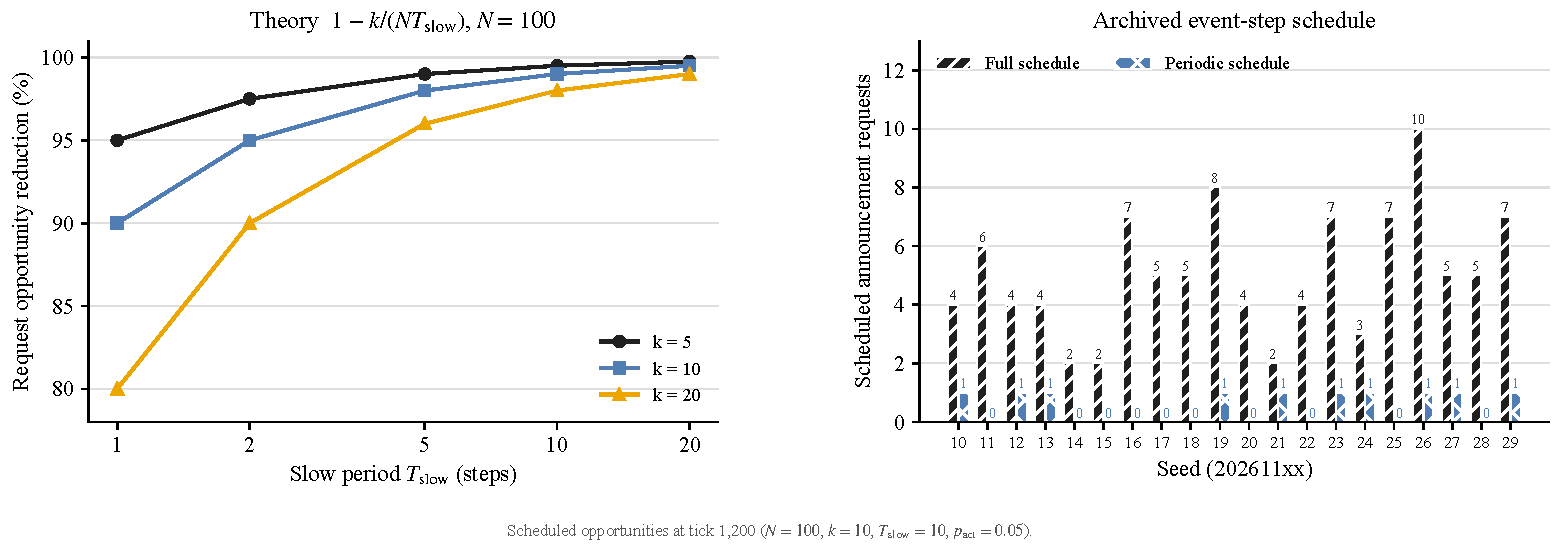
\includegraphics[width=\textwidth]{figures/schedule_exposure.pdf}
  \caption{Expected request reduction and announcement eligibility.}
  \label{fig:schedule_exposure}
 \end{subfigure}
 \par\medskip
 \begin{subfigure}{0.55\textwidth}
  \centering
  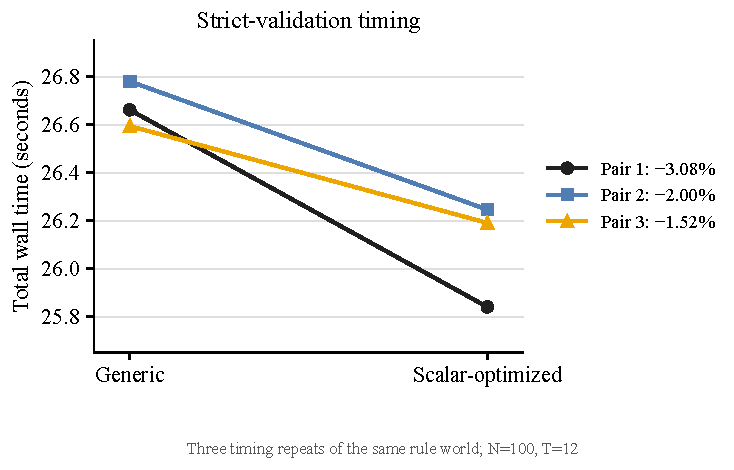
\includegraphics[width=\textwidth]{figures/engineering_timing.pdf}
  \caption{Paired wall-clock time for two strict validators.}
  \label{fig:timing_supp}
 \end{subfigure}
 \caption{Schedule and validator diagnostics. (a) The left panel varies the period $T_{\mathrm{slow}}$ and the slow group size $k$ at $N=100$ over horizons divisible by the period. The right panel counts active agents eligible to send the announcement at release. (b) Each line connects the generic and scalar-optimized timings for the same rule world.}
 \Description{Expected request reduction by schedule, announcement eligibility for 20 seeds, and paired validation timings.}
\end{figure*}


\end{document}
